This chapter describes how to simulate from our multiGLMM and describes
the performed simulation studies. The general simulation procedure is
addressed in \autoref{cap:simu}. In \autoref{cap:data} the simulation
studies are presented in detail.

\section{SIMULATING FROM THE MODEL}
\label{cap:simu}

Being able to simulate data from a model is a key task, fundamental to
assess the finite-sample properties and the estimation procedure
liability of a given statistical model. The step-by-step describing the
simulation procedure of our multiGLMM is presented on Algorithm
\autoref{alg:algo}, following the model hierarchical structure
stipulated in \autoref{eq:model}.

\begin{algorithm}[H]
 \caption{SIMULATING FROM A \(\text{multiGLMM}\) FOR CLUSTERED COMPETING
          RISKS DATA}
 \label{alg:algo}
 \begin{algorithmic}[1]
  \State
   Set \(J\), the number of clusters
  \State
   Set \(n_{j}\), the number of cluster elements
   \Comment{can be of different sizes}
  \State
   Set \(K-1\), the number of competing causes of failure
  \State
   Set the model parameter values \(\bm{\theta} =
   [\bm{\beta}~\bm{\gamma}~\bm{w}~\bm{\sigma^{2}}~\bm{\varrho}]^{\top}\)
  \State
   Sample \(J\) latent effect vectors from a
   \(\text{Multivariate Normal}_{(K-1)\times(K-1)}(
      \bm{0},~\Sigma(\bm{\sigma^{2},\varrho})
     )\)
  \State
   Set \(\delta\)
   \Comment{maximum follow-up time}
  \State
   Set the failure times \(t_{ij}\)
  \State
   Compute the competing risks probabilities
   \begin{align*}
    p_{kij} &=
    \frac{\exp\{\bm{x}_{kij}\bm{\beta}_{kj} + u_{kj}\}}{
          1 +
          \sum_{m=1}^{K-1}\exp\{\bm{x}_{mij}\bm{\beta}_{mj} + u_{mj}\}
         }\\
    &\times w_{k}\frac{\delta}{2\delta t_{ij} - 2t_{ij}^{2}}~
     \phi\left(w_{k}
      \text{arctanh}\left(\frac{t_{ij}-\delta/2}{\delta/2}\right) -
      \bm{x}_{kij}\bm{\gamma}_{kj} - \eta_{kj}
     \right),\\
    \text{Censorship}: \quad
    p_{Kij} &=
    1 - \sum_{k=1}^{K-1} p_{kij}, \quad k = 1,~2,~\dots,~K-1
   \end{align*}
  \State
   Sample \(J\times n_{j}\) vectors from a
   \(\text{Multinomial}(p_{1ij},~p_{2ij},~\dots,~p_{Kij})\)
  \State
   If \(t_{ij} = \delta\), moves to class K
   \Comment{any failure at time \(\delta\) is a censorship}
  \State
   \Return
    multinomial vectors and their respective failure/censoring times
 \end{algorithmic}
\end{algorithm}
\vspace{-1cm}
\begin{footnotesize}
  \begin{center}
    SOURCE: The author (2021).
  \end{center}
\end{footnotesize}

The model described in \autoref{eq:model} is in a general form, allowing
for varying coefficients between clusters. However, we focus on a
simpler structure with just fixed intercepts. Fixing the latent effects
in its distribution mean, zero, and using the following fixed effects
configuration for two competing causes of failure
\begin{align}
 \bm{\beta} &= [-2~~~1.5]^{\top}\nonumber\\
 \bm{\gamma} &= [1.2~~~1]^{\top}\label{eq:fixedconfig}\\
 \bm{w} &= [3~~~5]^{\top}\nonumber,
\end{align}
we get the CIF's and failure probabilities (CIF derivatives w.r.t. time
\(t\), dCIF) presented respectively in \autoref{fig:datasimucif}.

\begin{figure}[H]
 \setlength{\abovecaptionskip}{.0001pt}
 \caption{CUMULATIVE INCIDENCE FUNCTIONS (CIF) AND RESPECTIVE
          DERIVATIVES (\(\text{dCIF}\)) W.R.T. TIME FOR A MODEL WITH
          TWO COMPETING CAUSES OF FAILURE, WITHOUT COVARIATES, LATENT
          EFFECTS IN ZERO, AND FIXED EFFECTS IN
          \autoref{eq:fixedconfig}}
 \vspace{0.2cm}\centering
 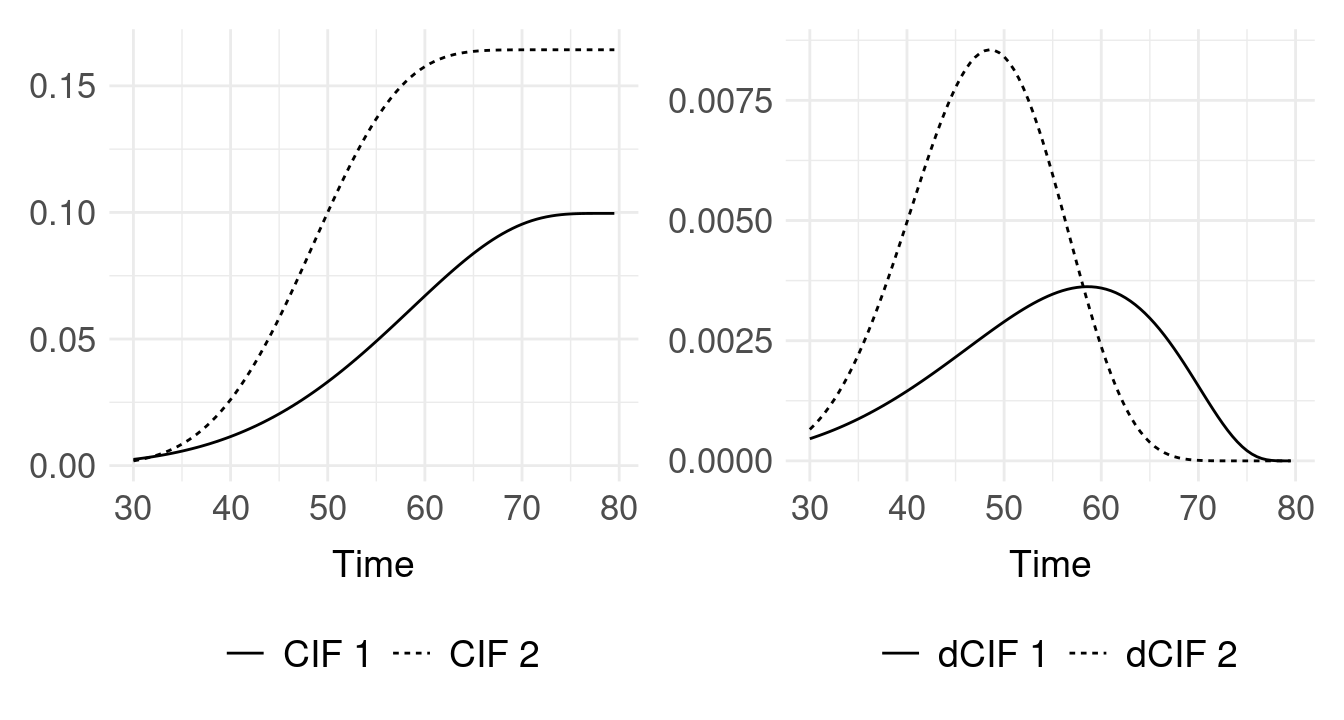
\includegraphics[width=0.8\textwidth]{datasimucif-1.png}\\
 \begin{footnotesize}
  SOURCE: The author (2021).
 \end{footnotesize}
 \label{fig:datasimucif}
\end{figure}

By adding a complete latent structure,
\begin{equation}
 \begin{bmatrix} u_{1}\\u_{2}\\\eta_{1}\\\eta_{2} \end{bmatrix}
 \sim\text{Multivariate Normal}
 \left(\begin{bmatrix} 0\\0\\0\\0 \end{bmatrix},
       \begin{bmatrix}
        1&0.4&-0.5& 0.4\\
         &  1& 0.4&-0.3\\
                &&1&0.4\\
                   &&&1
       \end{bmatrix}
 \right),\label{eq:latentconfig}
\end{equation}
we are able to apply Algorithm \autoref{alg:algo} and generate a
complete model sample with 50000 clusters of size two (pairs),
summarized in \autoref{fig:datasimu}. The \texttt{R} function written to
simulate the data is available in \autoref{cap:appendixC}.

Varying the parameters configuration we are able to build basically any
CIF's format. However, its dCIF will be always small i.e., the generated
probabilities for the failure causes will always be (really) small,
passing all the probability mass to the censorship class. Low
probabilities imply few failures, making the multiGLMM even harder to
fit. All these behaviors are seen in \autoref{fig:datasimu}.

\begin{figure}[H]
 \setlength{\abovecaptionskip}{.0001pt}
\caption{HISTOGRAMS FOR SIMULATED PROBABILITIES WITH RESPECTIVE OUTPUT
          PCERCENTAGES AND FAILURE TIMES FOR A MODEL WITH TWO COMPETING
          CAUSES AND 50000 CLUSTERS OF SIZE TWO. THE SIMULATION FOLLOWED
          ALGORITHM \autoref{alg:algo} GUIDELINES WITH PARAMETER
          CONFIGURATIONS SPECIFIED IN \autoref{eq:fixedconfig}
          AND \autoref{eq:latentconfig}}
\vspace{0.2cm}\centering
 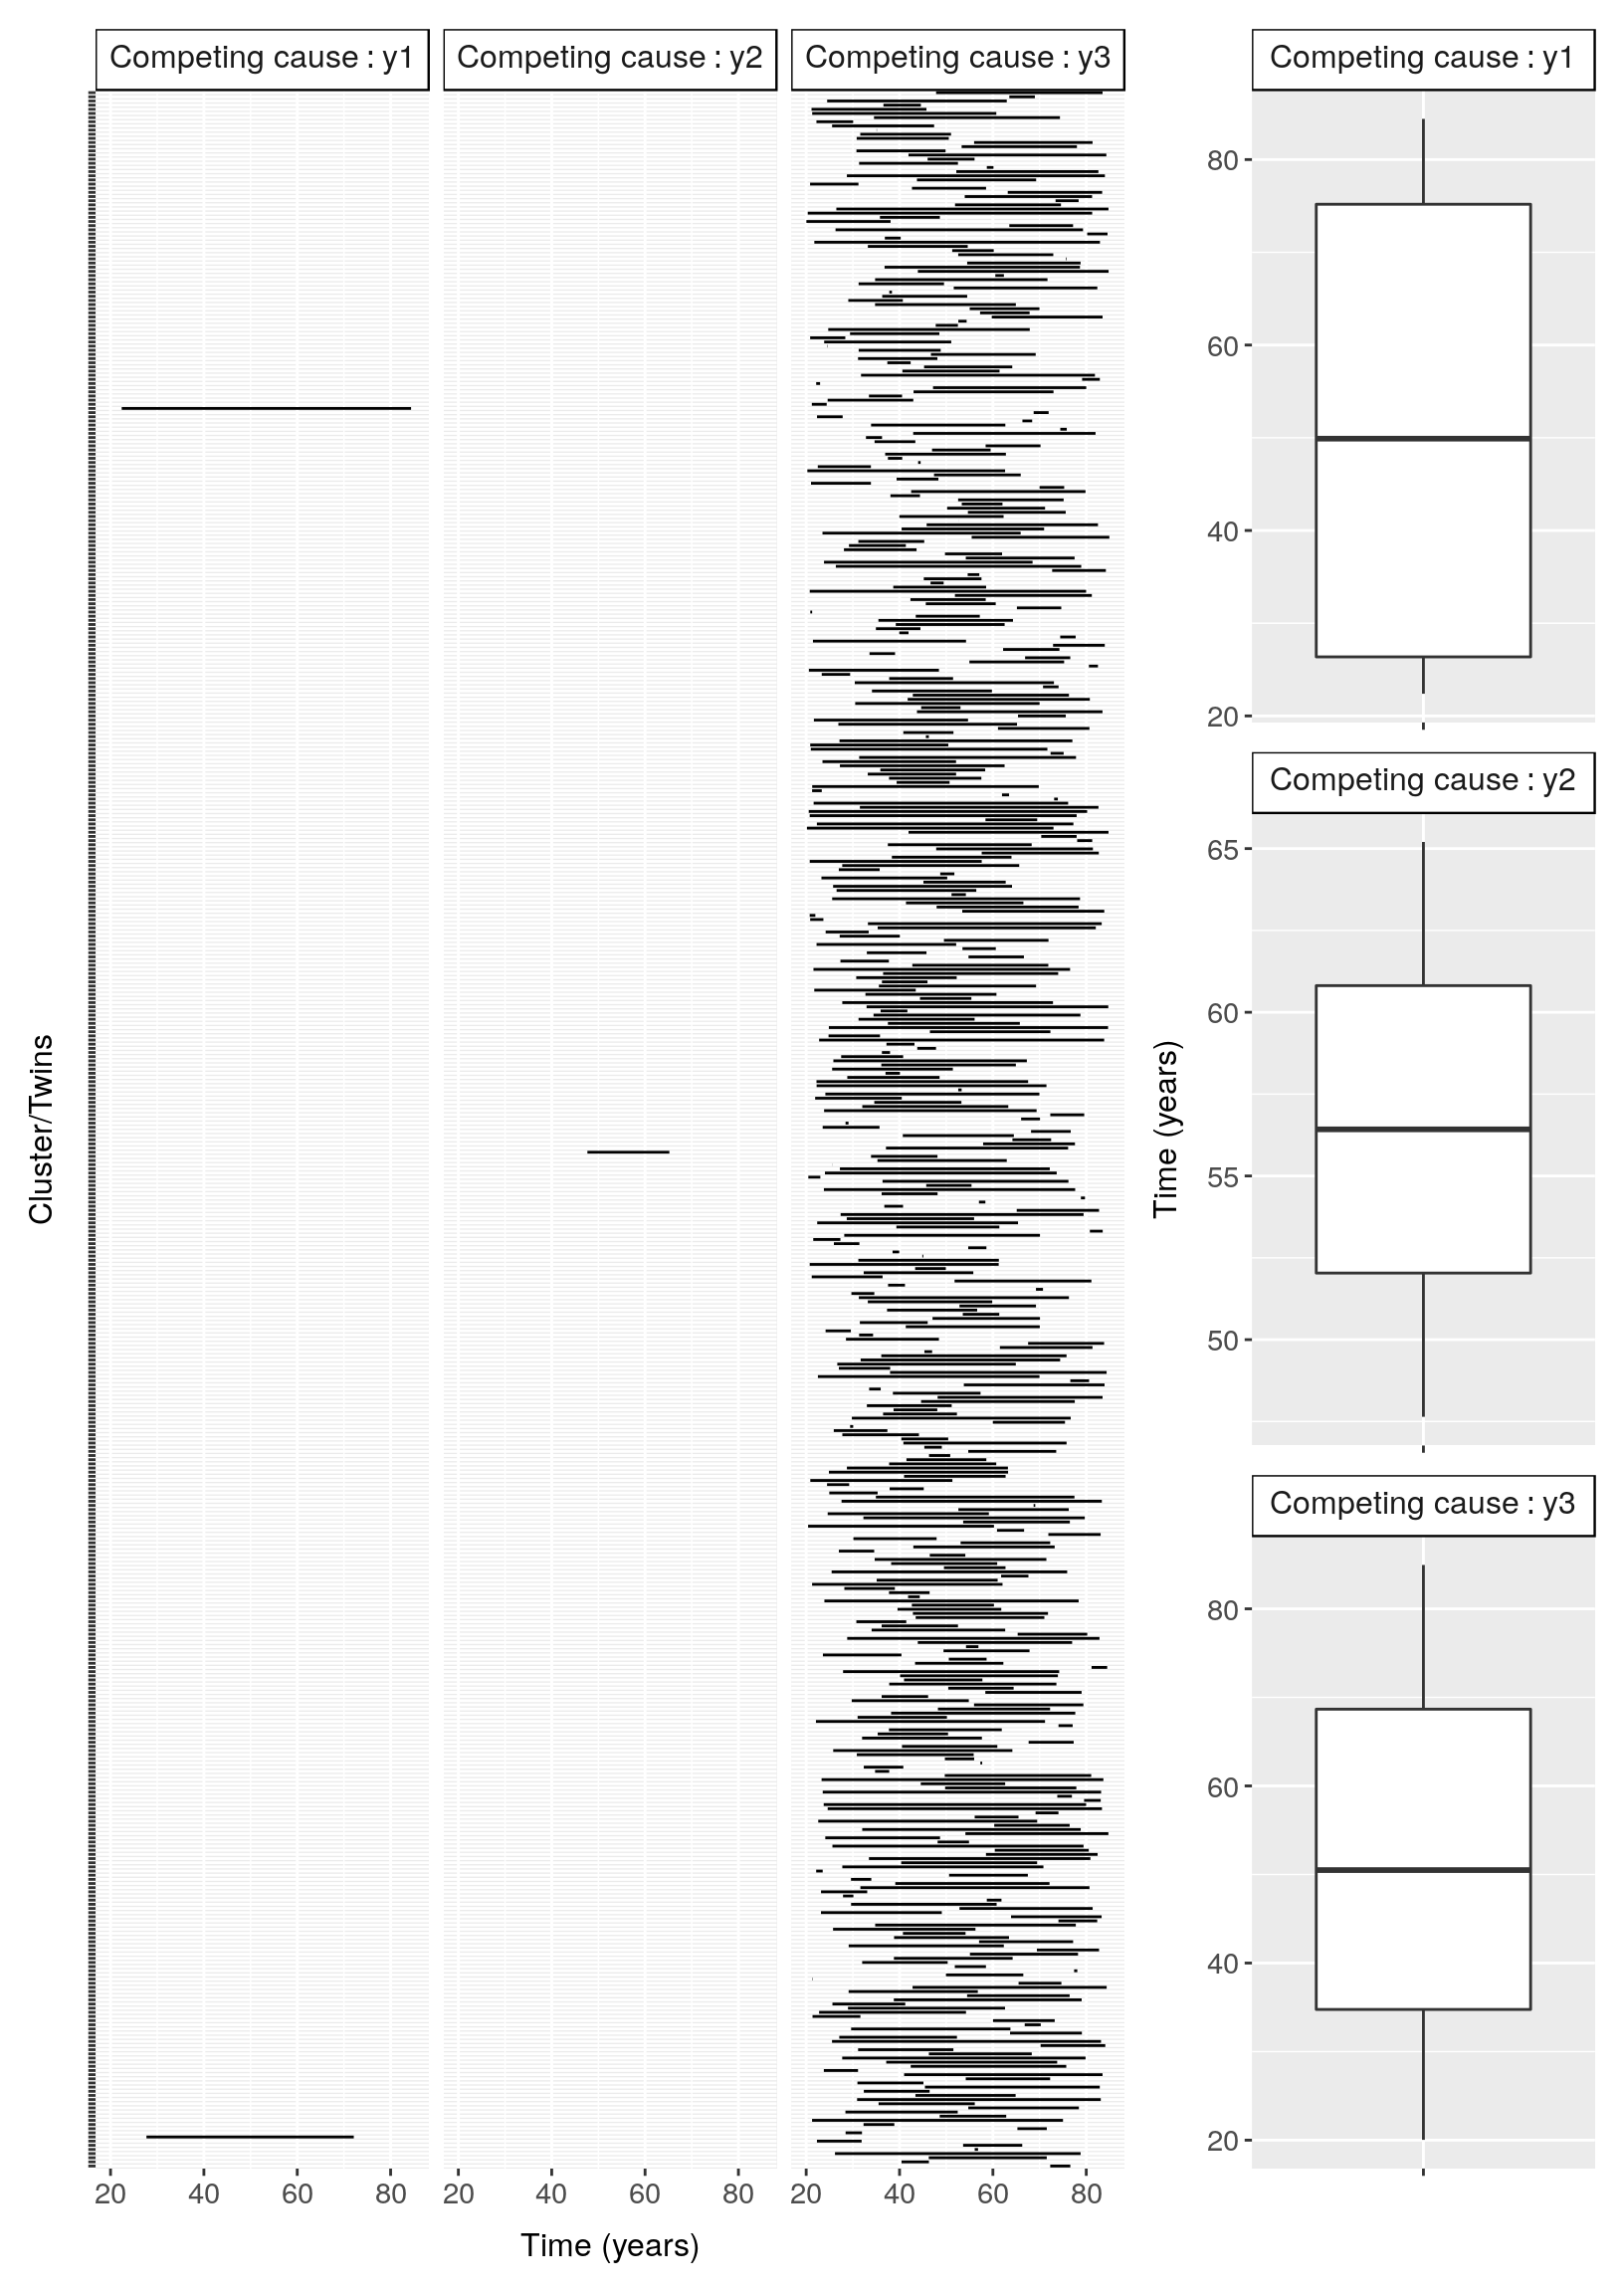
\includegraphics[width=\textwidth]{datasimu-1.png}\\
 \begin{footnotesize}
  SOURCE: The author (2021).
 \end{footnotesize}
 \label{fig:datasimu}
\end{figure}

Thinking of epidemiological or public health problems, the reasonable
CIF behaviors are the ones presented in \autoref{fig:datasimucif}. In
the simulation routine, the failure/censorship times are based on the
random sampling of values between 30 and 80-time units. Another approach
could be performing this random sampling by age group, to have something
similar to a realistic population pyramid. However, by performing some
tests we saw that having a realistic CIF is enough. Even with a uniform
time distribution, the failure times will not be uniform, as the CIF
curves impose their form. We can see this happening in the bottom graphs
of \autoref{fig:datasimu}.

\citeonline{SCHEIKE} does something different through the sampling of
the censorship times from a \(\text{U}(0,~\delta)\), the sampling of
\(\varsigma\sim\text{U}(0,~1)\), and the computation of the
cause-specific failure times by solving
\[
 \varsigma =
 \Phi\left(w_{k}
           \text{arctanh}\left(\frac{t_{ij}-\delta/2}{\delta/2}\right) -
           \bm{x}_{kij}\bm{\gamma}_{k} - \eta_{kj}
     \right)
 \quad\text{for}\quad t_{ij},
\]
with \(i\) being the subject, \(j\) the cluster, and \(k\) the failure
cause. This approach implies a parametric form for the failure times,
which we do not know if holds in the real world.

\section{SIMULATION STUDIES DESIGN}
\label{cap:data}

To stress the model and check the paramters identifiability, we propose
seventy-two scenarios. All scenarios with two competing causes. Thus, a
three classes multinomial distribution.

We consider two CIF scenarios, in summary, a low and a high CIF
scenario. The parameter configurations are presented together with their
curves in \autoref{fig:twodiffcifs}. As mentioned before, independent of
the configuration the censorship level is basically the same.

\begin{figure}[H]
 \setlength{\abovecaptionskip}{.0001pt}
 \caption{CUMULATIVE INCIDENCE FUNCTIONS (CIF) FOR A MODEL WITH TWO
          COMPETING CAUSES OF FAILURE, WITHOUT COVARIATES, AND LATENT
          EFFECTS IN ZERO}
 \vspace{0.2cm}\centering
 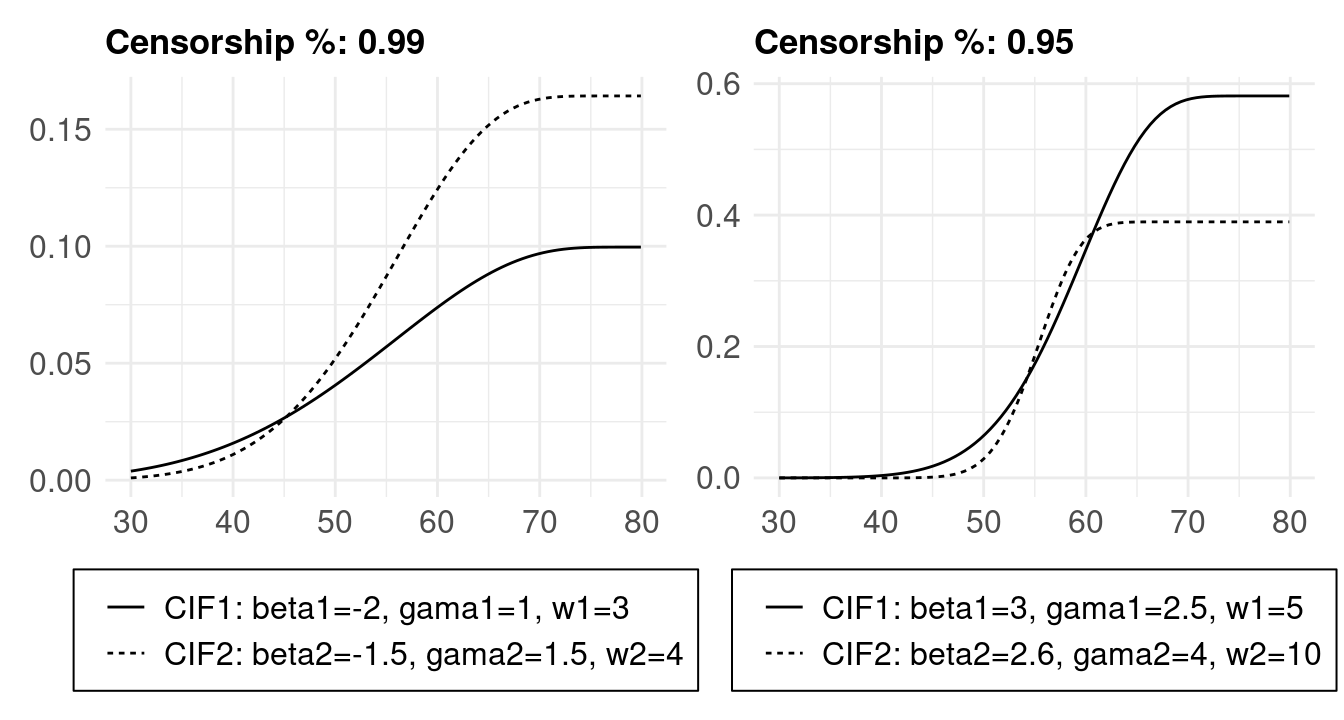
\includegraphics[width=0.8\textwidth]{twodiffcifs-1.png}\\
 \begin{footnotesize}
  SOURCE: The author (2021).
 \end{footnotesize}
 \label{fig:twodiffcifs}
\end{figure}

We use four multiGLMMs, that can be discriminated by their latent effect
structures.
\[
 \Sigma = \begin{bmatrix} R & C\\ C^{\top} & T \end{bmatrix}
 \quad~\text{with}~\quad
 R = \begin{bmatrix} 1.0 & 0.1\\ & 0.6 \end{bmatrix},\quad
 T = \begin{bmatrix} 0.7 & 0.2\\ & 0.9 \end{bmatrix},\quad
 C = \begin{bmatrix} -0.5 & 0.3\\ 0.3 & -0.4 \end{bmatrix}.
\]
They are
\begin{description}
 \item[risk model] A model with latent effects only on the risk level
      i.e., \(\Sigma_{~2\times2} = R\);

 \item[time model] A model with latent effects only on the trajectory
      time level i.e., \(\Sigma_{~2\times2} = T\);

 \item[block-diag model] A model with latent effects on the risk and
      trajectory time level only i.e., \(\Sigma_{~4\times4} =
      \text{diag}(R, T)\);

 \item[complete model] A model with a \textit{complete} latent effects
      structure i.e, \(\Sigma_{~4\times4} = \Sigma\).
\end{description}
All models are based on some decomposition of the matrix
\[
 \Sigma = \begin{bmatrix} R & C\\ C^{\top} & T \end{bmatrix}
        = \begin{bmatrix}
            1.0 &  0.1 & -0.5 &  0.3\\
            0.1 &  0.6 &  0.3 & -0.4\\
           -0.5 &  0.3 &  0.7 &  0.2\\
            0.3 & -0.4 &  0.2 &  0.9
          \end{bmatrix}.
\]
Propose a \(4\times4\) matrix like this is not so simple since we should
not only look at the values coherence. The matrix should also be
positive-definite, and more than that, the submatrices \(R\), \(T\),
and \(\text{diag}(R, T)\), should also be positive-definite since they
are also used as variance-covariances matrices.

Three sample sizes are used, 5000; 30000; and 60000 data points. They
are combined with three cluster sizes, size 2; size 5; and size 10
clusters. Thus,
\begin{minipage}{\textwidth/3}
 \begin{align*}
          &\textit{5000 data points},\\
  \bullet~&\text{2500 clusters of size 2}\\
  \bullet~&\text{1000 clusters of size 5}\\
  \bullet~&\text{500 clusters of size 10}
 \end{align*}
\end{minipage}%
\begin{minipage}{\textwidth/3}
 \begin{align*}
          &\textit{30000 data points},\\
  \bullet~&\text{15000 clusters of size 2}\\
  \bullet~&\text{6000 clusters of size 5}\\
  \bullet~&\text{3000 clusters of size 10}
 \end{align*}
\end{minipage}%
\begin{minipage}{\textwidth/3}
 \begin{align*}
          &\textit{60000 data points},\\
  \bullet~&\text{30000 clusters of size 2}\\
  \bullet~&\text{12000 clusters of size 5}\\
  \bullet~&\text{6000 clusters of size 10}
 \end{align*}
\end{minipage}\\

Besides the sample size per se, by increasing it we also increase the
number of Laplace approximations to be performed since each cluster
implies a Laplace approximation. This affects hugely the computational
time.

In summary, we have

Two CIF configurations, four latent effect structures, three sample
sizes, and three cluster sizes; \(2 \times 4 \times 3 \times 3 = 72\)
scenarios. For each scenario, we simulate 100 samples and fitted the
corresponding model.

% END ==================================================================
